\chapter{System implementation}

In this chapter we will discuss the actual implementation of the original idea
behind Linkero: a brand monitoring case management application. We will start
from the architecture in order to show a general snapshot of the system, before
talking in details about every single component, the technology that was
chosen and reasons behind. We will follow with use cases and
system requirements, to conclude with class diagram, database structure and some
code samples.

\section{System architecture}
The system achitecture represented in figure \ref{fig:sysarch} provides an
overview of all different applications that work together to perform the main
system functionalities.

\begin{figure}[h!]
\centering
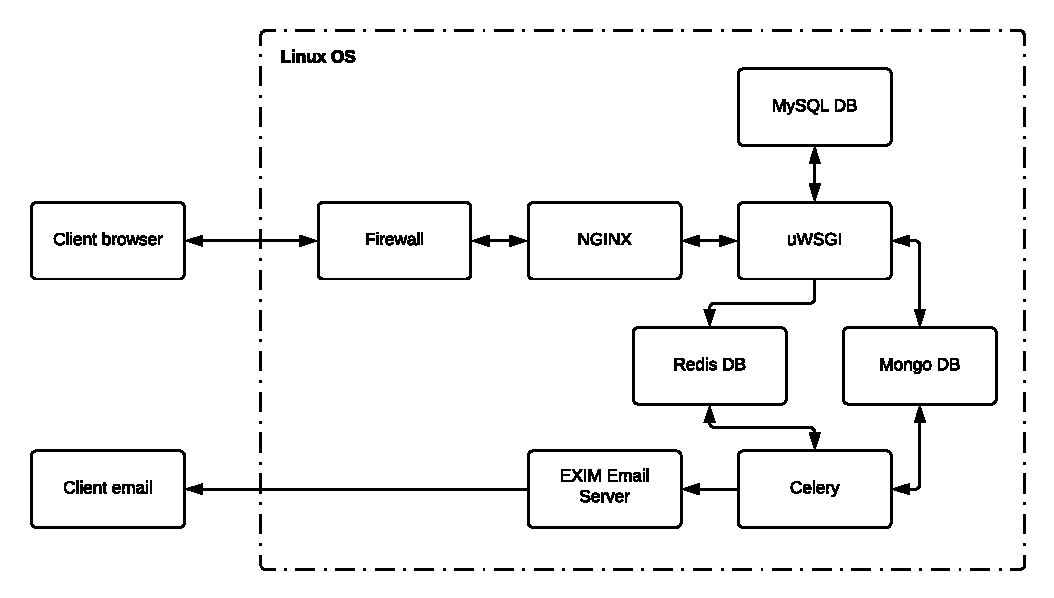
\includegraphics[scale=0.7]{imgs/SystemArchitecture.pdf}
\caption{Linkero system architecture}
\label{fig:sysarch}
\end{figure}

As shown in the figure, client browser and client email are considered part of
the system: the former becuase some functionalities are passed to the client to
run locally in the form of JQuery functions, and the latter because it represent
the final destination of data files generated bythe system.

Linux is the operating system running on a Virtual Private Server, that manages
all other applications. The first point of entry is the Firewall, which monitors
all requests knocking ports 22, 80 and 443.

NGINX is the web server, reverse proxy server \cite{WikiNginx}, which receives
HTTP requests and assigns them to the correct internal web server.

uWSGI is the web server that runs Python scripts, in the words of its
developers: ``uWSGI itself is a vast project with many components, aiming to
provide a full software stack for building hosting services'' \cite{RtduWsgi}.

Python scripts from within uWSGI can make calls to three databases. MySQL keeps
information about users registration details, passwords, and access logs. Mongo
DB instead is used to store all the data generated by users with their queries.
Finally Redis DB simply stores information about tasks that have been scheduled
and that will run independently from uWSGI's scripts.

Celery is another server running Python scripts scheduled by the main web
server. It does so by regularly checking in Redis if any new task has been
logged, and if that's the case it will execute each task sequentially.

Finally the email server is only called for outgoing emails, to deliver a copy
of all the data collected in a .csv file attached to the email.

\section{Technologies}

The overall system was not written from scratch, there are many free and
open-source applications that were assembled in order for the system to work.

\subsection{Server operating system}
Linkero is hosted on a Virtual Private Server provided by the company Linode
\texttrademark. We chose the smallest package offering 1 GB Ram, 1 CPU Core and
25 GB of SSD storage at \textdollar 5.00 USD a month.

The plan offers different operating systems to chose from, and Linux Debian is
the OS that was picked for this project. There are several advantages to us a
Linux distribution:
\begin{itemize}
  \item Linux is a very lightweight system, which can run on hardware with even
  smaller resources than the ones available for this project;
  \item Linux is mantained by a global community who prioritize reliability and
  security over functionalities;
  \item Linux is opesource system, which means that its code can be read by
  anyone, increasing the chances of finding bugs and vulnerabilities, which is
  to say that Linux is very secure;
  \item Linux is also one of the most popular server technologies, guaranteeing
  that a system designed for Linux can access and be transferred to a vast
  public already using Linux;
  \item the Debian distribution development cycle emphasizes stability over
  innovation, offering products that are well tested before being published;
  \item installation and use are free and allowed under the GNU General Public
  License, making it ideal for a small budget project;
  \item the Debian distribution is one of the most rich in extra applications
  ready to be installed from their officila directories \cite{Debian}.
\end{itemize}

All the reasons above make Linux Debian the ideal candidate for this project.

\subsection{Web application framework}

As mentioned before, the main business logic in this project is written in
Python and runs on a uWSGI web server. However the actual set of objects and
functions that constitute a web application have been developed using Django.
Django is a ``web framework for perfectionists with deadlines'', quoting from
Django developers' tagline \cite{Django}. There are several reasons that make
Django a good candidate for this project:
\begin{itemize}
  \item the web development framework is freely distributed under the BSD
  Licence;
  \item Django offers object-relational mapping classes designed to interact
  directly with a relational database using Python APIs, simplifying
  interactions and code that involves data retrival and manipulations with a SQL
  database;
  \item Django has already built-in user authentication and authorization and session management
  support, along with a pre-installed admin console with basinc
  functionalities;
  \item Django comes with several security features to prevent web-specific
  attack, such as: cross-site scripting, cross-site request forgery,
  SQL-injection, clickjacking;
  \item Django is designed with scalability in mind: it enforces strict
  separation between application layer and database layer, so that new hardware
  can be added with no costly impact due to reconfiguration.
\end{itemize}

Chosing Django also means being able to access all the Python libraries
available for data analysis, data mining and system administration.

\subsection{Databases}
There are three different databases that support all the data needs of this
project.

\subsubsection{MariaDB}
MariaDB is a version of MySQL that forket from the original development in order
to remain free under the GNU GPL licence. There is no special reason to prefer
this relational database over the parent MySQL, other than it is the default
version available in the original Debian repositories, since all Debian software
is protected by GNU GPL.

MariaDB is used as default server for user authentication and session
management, and to keep logs of user log-in, user IPs and browsing activity.


\subsubsection{MongoDB}

\subsubsection{Redis}

\subsection{Web engine}
NGINX was chosen to serve the pages of this application.

\subsection{Firewall}

\subsection{Celery}

\section{Development methodology}

\section{Use cases}

\begin{figure}[h!]
\centering
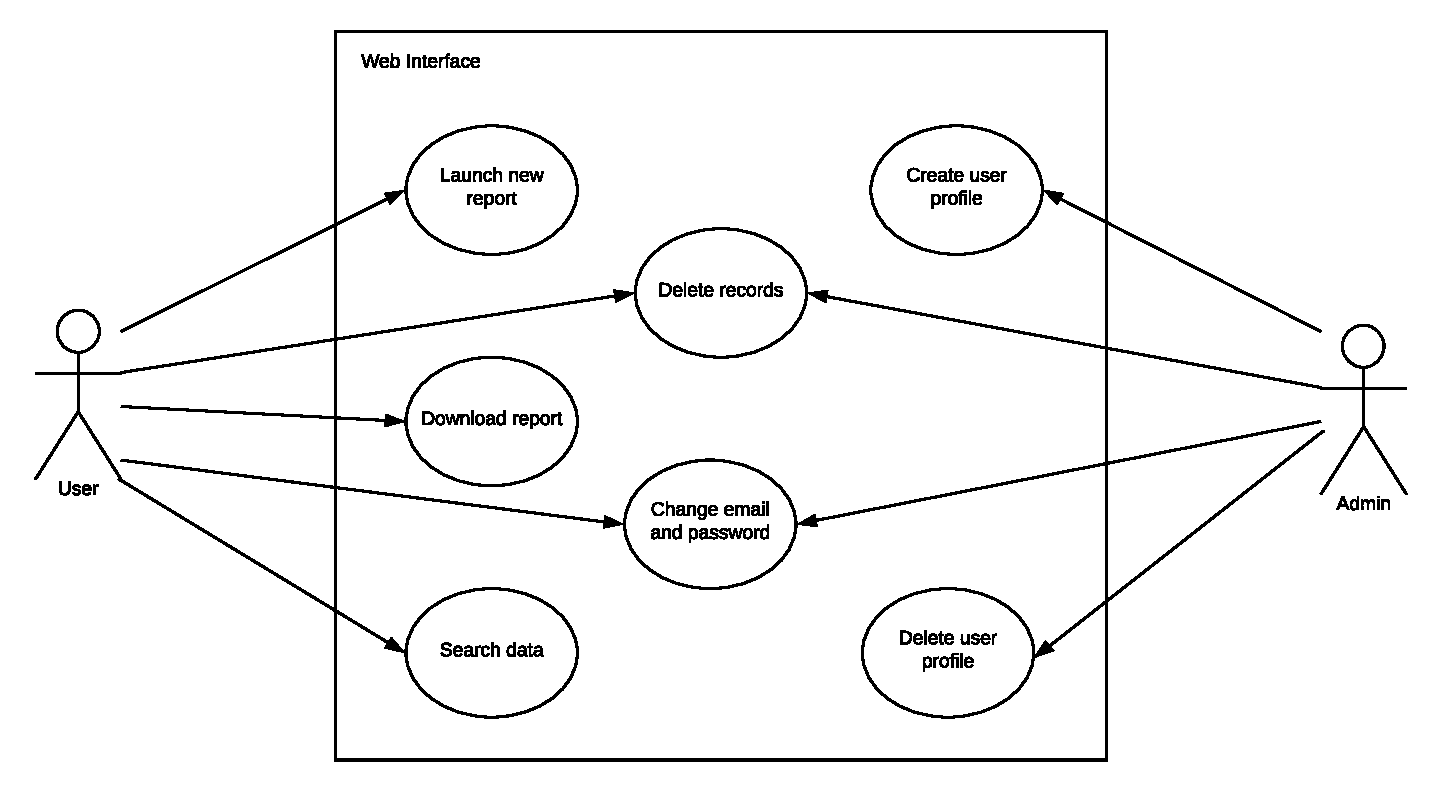
\includegraphics[scale=0.4]{imgs/UseCasesDiag.pdf}
\caption{Use cases diagram}
\label{fig:sysarch}
\end{figure}

\section{Requirements}

\subsection{Functional requirements}

\subsection{Non-functional requirements}

\begin{itemize}
  \item security
  \item scalability
  \item maintainability
\end{itemize}

\subsection{User requirements}

\subsection{Requirements analysis}

\section{Sequence diagrams}

\begin{figure}[h!]
\centering
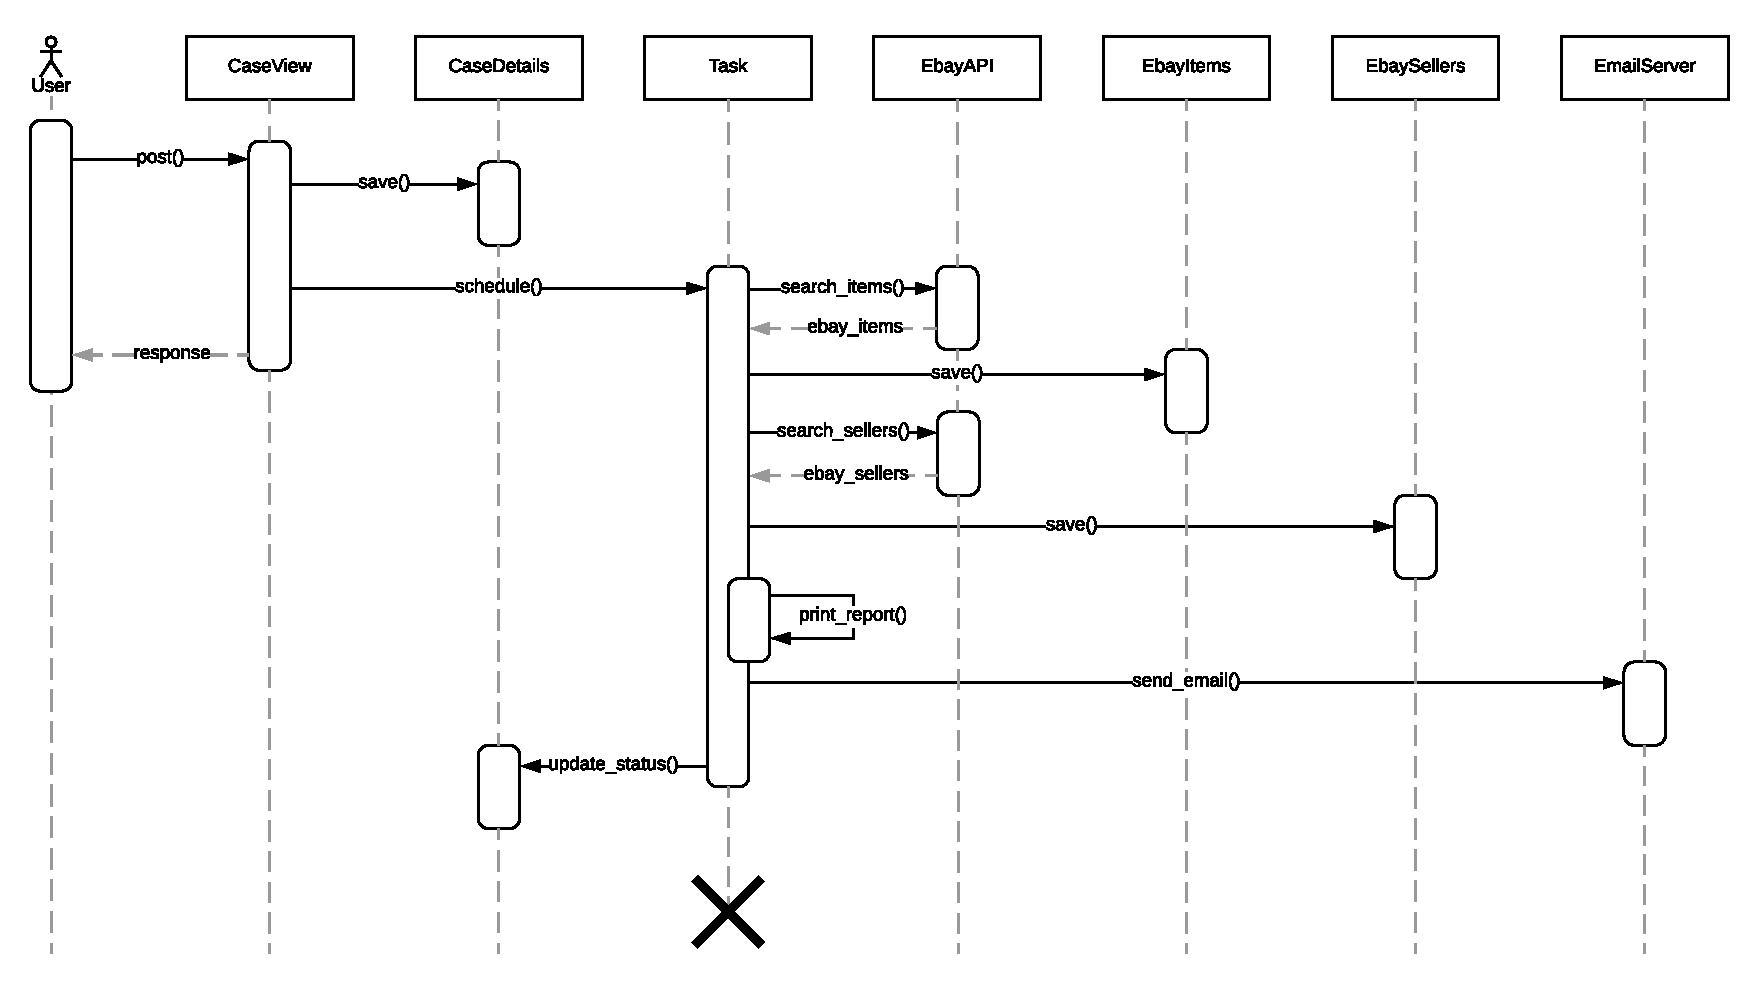
\includegraphics[angle=90, scale=0.7]{imgs/SequenceDiagram.pdf}
\caption{Launch report sequence diagram}
\label{fig:sysarch}
\end{figure}

\section{Code samples}
